\documentclass[11pt,twoside,openright]{report}
\usepackage[utf8]{inputenc}   % Encodage entrée
\usepackage[T1]{fontenc}      % Encodage des polices
\usepackage{graphicx}         % Images
\usepackage[usenames,svgnames,table]{xcolor} % Couleurs
\usepackage{tocloft}          % Gestion des tables
\newlistof{listing}{lol}{Liste des extraits de code}
\usepackage[chapter,newfloat]{minted}  % Mise en forme de code source
\usepackage{framed}           % Cadres et bordures
\usepackage[francais]{babel}  % Langue
\usepackage{amsmath}          % Symboles maths

\usepackage[autolanguage,np]{numprint} % Formatage des nombres
\usepackage{caption}          % Légendes
\usepackage{sidecap}          % Légende latérale
\usepackage{subcaption}       % Légendes des sous-figures
\usepackage{enumitem}         % Formatage des listes à puces
\usepackage{blindtext}        % Texte caché
\usepackage[nobottomtitles]{titlesec} % Formatage des chapitres
\usepackage[a4paper]{geometry}    % Mise en page
\usepackage[hidelinks]{hyperref}  % Liens
\usepackage{fancyhdr}             % Headers & footers
\usepackage{tcolorbox}              % Coloration des cellules de tableaux
\usepackage[xindy,toc]{glossaries}  % Glossaire
\usepackage[sfdefault]{quattrocento}

\usepackage{chngcntr}               % Gestion des compteurs
\usepackage{emptypage}              % Pages blanches sans header ni footer
\counterwithout{footnote}{chapter}  % Numérotation des notes de pied de page indépendante du chapitre (pas de RAZ)

% Paramètres affichage des liens et métadonnées PDF
\hypersetup{
  bookmarks=false,         % show bookmarks bar?
  unicode=false,          % non-Latin characters in Acrobat’s bookmarks
  pdftoolbar=false,        % show Acrobat’s toolbar?
  pdfmenubar=false,        % show Acrobat’s menu?
  pdffitwindow=false,     % window fit to page when opened
  pdfstartview={FitH},    % fits the width of the page to the window
  pdftitle={},    % title
  pdfauthor={},     % author
  pdfsubject={},   % subject of the document
  pdfcreator={PDFLaTeX},   % creator of the document
  pdfproducer={LaTeX}, % producer of the document
  pdfnewwindow=true,      % links in new window
  colorlinks=false,       % false: boxed links; true: colored links
  linkcolor=red,          % color of internal links (change box color with linkbordercolor)
  citecolor=green,        % color of links to bibliography
  filecolor=magenta,      % color of file links
  urlcolor=cyan           % color of external links
}

% Import des paramètres de mise en forme de code source.
% \usepackage{upquote}
\usepackage{textcomp}
\usepackage{minted}
\usepackage{inconsolata}
\usepackage{MnSymbol}

\newminted[cppcode]{c++}{
  breaklines             = true,
  frame                  = single,
  breakautoindent        = true,
  breaksymbolleft        = $\lhookrightarrow$,
  breaksymbolindentleft  = 10pt,
  breaksymbolsepleft     = 2pt,
  breaksymbolright       = $\rhookleftarrow$,
  breaksymbolindentright = 10pt,
  breaksymbolsepright    = 2pt,
  texcomments            = true
}


\newmintedfile[cppfile]{c++}{
  linenos                = true,
  tabsize                = 2,
  breaklines             = true,
  frame                  = single,
  breakautoindent        = true,
  breaksymbolleft        = $\lhookrightarrow$,
  breaksymbolindentleft  = 10pt,
  breaksymbolsepleft     = 2pt,
  breaksymbolright       = $\rhookleftarrow$,
  breaksymbolindentright = 10pt,
  breaksymbolsepright    = 2pt,
  label                  = Code C++,
  texcomments            = false
}

\newmintinline[cppinline]{c++}{
breaklines = true
}

%%%%%%%%%%%%%%%%%%%%%%%%%%%%%%%%%%%%%%%%%%
%        PARAMETRES DE METADONNEES       %
%%%%%%%%%%%%%%%%%%%%%%%%%%%%%%%%%%%%%%%%%%
\newcommand{\titre}{Conception d'un solveur pour l'interception de mobiles}
\newcommand{\sujet}{Projet ZZ3}
\newcommand{\sujetLong}{Projet de 3\ieme{} année}
\newcommand{\auteur}{Aurélie PERES, Pierre-Loup PISSAVY}
\newcommand{\dateRendu}{Mars 2017}

% Paramètres de métadonnées du PDF
\hypersetup{
  pdftitle={\sujetLong{} - \titre},
  pdfsubject={\sujet},
  pdfkeywords={},
  pdfauthor={\auteur}
}

%%%%%%%%%%%%%%%%%%%%%%%%%%%%%%%%%%%%%%%%%%
%        MISE EN PAGE DU DOCUMENT        %
%%%%%%%%%%%%%%%%%%%%%%%%%%%%%%%%%%%%%%%%%%
\geometry{left=3cm,right=2cm,top=2.5cm,bottom=2.5cm}

\frenchbsetup{StandardLists=true}
\npthousandsep{~}

\edef\hc{\string:}

\newcommand{\hsp}{\hspace{10pt}}
\newcommand{\blankpage}{\newpage \thispagestyle{empty} \addtocounter{page}{-1} \null \newpage}

\titleformat{\chapter}[hang]{\color{gray}\huge\bfseries}{\thechapter\hsp{|}\hsp}{0pt}{\color{black}\huge\bfseries}
\renewcommand{\cftchapafterpnum}{\vspace{0pt}}
\setlength{\cftbeforechapskip}{.1ex}

% Pages de contenu
\fancypagestyle{IHA-fancy-style}{%
  \fancyhf{}%
  \fancyhead[RO]{\rightmark}
  \fancyfoot[RO]{\thepage}
  \fancyfoot[LO]{\titre}%
  \fancyhead[LE]{\leftmark}
  \fancyfoot[LE]{\thepage}
  \fancyfoot[RE]{ISIMA -- \sujetLong}%
  \renewcommand{\headrulewidth}{0.4pt}% Ligne de header
  \renewcommand{\footrulewidth}{0.4pt}% Ligne de footer
}
% Style de base: sert pour les nouveaux chapitres
\fancypagestyle{plain}{%
  \fancyhf{}%
  \fancyfoot[RO]{\thepage}%
  \fancyfoot[LO]{\titre}%
  \fancyfoot[LE]{\thepage}%
  \fancyfoot[RE]{ISIMA -- \sujetLong}%
  \renewcommand{\headrulewidth}{0pt}% pas de ligne de Header
  \renewcommand{\footrulewidth}{0.4pt}% ligne de footer
}
\captionsetup{labelfont=bf,textfont=it}
\captionsetup[table]{name=\textsc{Tableau}}

\newcommand{\TODO}[1]{\colorbox{red}{#1}}

%%%%%%%%%%%%%%%%%%%%%%%%%%%%%%%%%%%%%%%%%%
%        ENVIRONNEMENT POUR CODE         %
%%%%%%%%%%%%%%%%%%%%%%%%%%%%%%%%%%%%%%%%%%
\newenvironment{code}{\captionsetup{type=listing}}{}
\SetupFloatingEnvironment{listing}{%
  name={Code},
  fileext=lol}

\author{\auteur}
\date{\dateRendu}
\title{\titre}

%%%%%%%%%%%%%%%%%%%%%%%%%%%%%%%%%%%%%%%%%%
%        PARAMETRES DU GLOSSAIRE         %
%%%%%%%%%%%%%%%%%%%%%%%%%%%%%%%%%%%%%%%%%%
\setglossarystyle{long3col}       % Mise en page
\setlength{\glsdescwidth}{10cm}   % Ajustement
\makeglossaries                   % Calcul   % Import des paramètres
\newglossaryentry{cache}
{
	name=cache,
	first=cache\textsuperscript{$\ddagger$}, % Première occurrence marquée par le double obèle.
	firstplural=caches\textsuperscript{$\ddagger$},
	plural=caches,
	description={Une mémoire cache ou antémémoire est, en informatique, une mémoire qui enregistre temporairement des copies de données provenant d'une source, afin de diminuer le temps d'un accès ultérieur (en lecture) d'un matériel informatique (en général, un processeur) à ces données. \cite{wikipedia-cache}}%,
	%user1={Variante 1\textsuperscript{$\ddagger$}}
}    % Récupération des entrées du glossaire

\begin{document}
  \setlength{\parskip}{10pt}
  % 1ere de couverture
  \pagestyle{plain} % Page blanche
  \makeatletter
\begin{titlepage}
  \newcommand{\HRule}{\rule{\linewidth}{0.5mm}}
  \center
  
\includegraphics[width=6.4cm]{ISIMA_logo.pdf}
  \vspace{.5cm}

  % \thiswatermark{
  %   \begin{minipage}{\textwidth}
  %     \vspace{24cm}
  %     \begin{center}
  %     \rotatebox{45}{\scalebox{5}{\color{red!50!white}RAPPORT CONFIDENTIEL}}
  %     \end{center}
  %   \end{minipage}
  % }

  % \null\hfill
  % \begin{minipage}{.3\textwidth}
  % \begin{flushleft} \large
  %   Adresse entreprise
  % \end{flushleft}
  % \end{minipage}
  % \vspace{1cm}

  {\bfseries\Large Rapport d'ingénieur\\[.3cm]
  \sujetLong \\[.5cm]
  \large Filière Génie Logiciel\\[1cm]}
  \HRule \\[0.3cm]
  { \LARGE \bfseries \@title}\\ %[.3cm] %A activer si plusieurs lignes
  \HRule \\[1.5cm]

  \begin{flushleft} \Large \bfseries
    \emph{Présenté par:} \@author\\[1cm]
  \end{flushleft}
  \begin{minipage}[t]{0.52\textwidth}
    \begin{flushleft} \large
      Responsable ISIMA: Christophe DUHAMEL%\\[.5cm]
%      Responsable Entreprise: 
    \end{flushleft}
  \end{minipage}
  \hfill
  \begin{minipage}[t]{0.42\textwidth}
    \begin{flushleft} \large
      Soutenance: \@date\\[.5cm]

      %Durée du stage: 5 mois
    \end{flushleft}
  \end{minipage}\\[1.5cm]

  \vfill

  \begin{minipage}[c]{0.10\textwidth}
    \vfill
    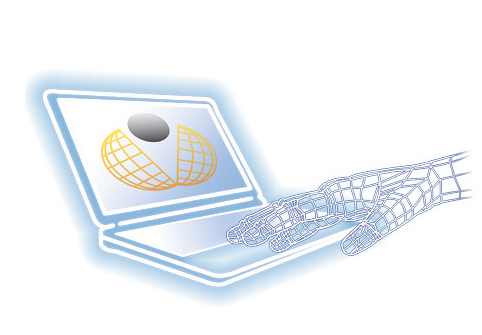
\includegraphics[width=\linewidth]{isima_main.png}
    \vfill \null
  \end{minipage}
  \begin{minipage}[b]{0.89\textwidth}
    \textbf{Institut Supérieur d'Informatique, de Modélisation et de leurs Applications}
    \vskip1mm
    {\color{NavyBlue}\hrule}
    \vskip3mm
    \begin{minipage}{0.78\textwidth}
      \textcolor{NavyBlue}{\large\textbf{www.isima.fr}}\\
      Campus universitaire des Cézeaux -- 1 rue de la Chebarde\\
      TSA 60125 -- CS 60026 -- 63178 Aubière CEDEX\\
      Tel (+33/0) 473 405 000 -- Fax (+33/0) 473 405 001
    \end{minipage}
    \hfill
    \begin{minipage}{0.20\textwidth}
      \raggedleft
      
\includegraphics[height=1.6cm]{UCA_logo.png}
    \end{minipage}
  \end{minipage} 

\end{titlepage}
\makeatother
  \blankpage

  \pagenumbering{roman}       % numérotation en chiffres romains
  
  % Remerciements
  \cleardoublepage
  \null
\vspace{4cm}
\begin{flushright}
	{\Large \bfseries Remerciements}
	\addcontentsline{toc}{chapter}{Remerciements}

	\vspace{1cm}

	\begin{minipage}{0.62\textwidth}
		Nous remercions Christophe Duhamel, responsable de notre projet, pour sa disponibilité tout au long du développement ainsi que pour ses nombreuses explications qui furent d'une aide constante et sans lequelles nous n'aurions pas pu mener ce projet à son terme.
	\end{minipage}

	\vspace{1cm}

	\begin{minipage}{0.62\textwidth}
		Remerciement 2
	\end{minipage}

\end{flushright}


  % Résumé + Abstract sur 1 page
  \cleardoublepage
  \section*{Résumé}
\addcontentsline{toc}{chapter}{Résumé}

L'identification d'objets mobiles est un problème d'optimisation courant pour les tournées de véhicules, doté de nombreuses applications. Par exemple, on peut l'utiliser pour modéliser et organiser des interventions de sécurité ou des opérations humanitaires. Dans les deux cas, le temps est une donnée critique et les solutions doivent maximiser le nombre de mobiles interceptés et minimiser le temps requis total. Ce problème nécessite donc une optimisation bi-critères et est appelé problème sélectif de tournées de véhicules avec dépendance de temps. Pour résoudre ce problème, nous avons implémenté deux heuristiques de construction pour générer des solutions réalisables, mais non optimales. Une politique de cache de données a été réalisée pour accélérer les heuristiques. Ensuite, des procédures de recherche locale ont été ajoutées pour déterminer les améliorations possibles d'une solution et une Vertical Neighbouhood Descent (VND) a été construite pour combiner ces méthodes. Puis deux métaheuristiques fondées sur un algorithme génétique à clés aléatoires et à multiples démarrages ont été utilisées pour générer de meilleures solutions sur les critères de temps et de quantité. Les algorithmes développés doivent être capables de fournir des solutions rapidement, ils ont donc été écrits dans le langage C++ et ont été calibrés avec des problèmes de taille réelle. Nous présentons les résultats de jeux de données connus et générés automatiquement. Les résultats montrent que la politique de cache de données a divisé le temps de calcul des heuristiques par dix. Plusieurs graphiques représentant les données dans l'espace et le temps sont fournis ainsi que le calibrage et la représentation des fronts de Pareto pour la comparaison et le classement des solutions générées. L'efficacité et la convergence des graphiques justifie les décisions stratégiques prises dans le processus de construction de la VND. Les résultats obtenus à la fin du projet confirment que les problèmes de tournées peuvent être résolus en utilisant des méthodes itératives de construction là où une résolution exacte échouerait ou mettrait énormément de temps à cause du très grand nombre de possibilités existantes. Ces résultats nous ont permis de valider une preuve de concept pour la prédiction du temps requis pour arrêter des trafiquants de drogues à bord de véhicules à grande vitesse.

\emph{Mots-clés: Aide à la décision, problème de tournées de véhicules, métaheuristique, Vertical Neighbourhood Descent, optimisation bi-critère.}

\section*{Abstract}
\addcontentsline{toc}{chapter}{Abstract}

Mobile objects identification is a common vehicle routing optimisation problem with several applications. For instance, it can be used to model and organise safety or humanitarian operations. In both cases, time may be critical and solutions must maximise the amount of visited mobiles and minimise the total needed time. This problem needs bi-criteria optimisation and is called an open vehicle routing problem with time dependency. To solve this problem, we implemented two route-building heuristics to generate feasible but not optimal solutions and a memory cache strategy was designed to speed-up the heuristics. Then, local search procedures were coded to look for improvements on the solutions and a Vertical Neighbourhood Descent was built to combine these procedures. After that, two metaheuristics based on a genetic algorithm with random keys and multi-start were used to generate better solutions on both time and amount criteria. The developed algorithms must be able to provide solutions quickly, so they were written using the C++ language and benchmarked with real-size problems. We present results of experiments on self-generated and well-known datasets. Results showed that the memory cache strategy divided the heuristic computation by ten. Several graphical representations for temporal and spatial dimensions were also provided along with a benchmark and Pareto frontiers charts to compare and rank the generated solutions. Efficiency and convergence charts justified the strategic decisions taken in the Vertical Neighbourhood Descent building process. The results obtained at the end of this project confirm that routing problems can be solved using constructive and iterative methods because of the large amount of possibilities on which an exact solver would fail or need an extremely long time to end. These results made it possible for us to validate a proof of concept in predicting how much time is needed to arrest drug smugglers on "go-fast" races.

\emph{Keywords: Decision support, Vehicle Routing Problem, Metaheuristic, Vertical Neighbourhood Descent, Bi-criteria optimisation.}


  % Table des matières, illustrations, tableaux, listings
  \cleardoublepage
  \pagestyle{IHA-fancy-style}
  \newlength{\currentparskip}
\setlength{\currentparskip}{\parskip}
\setlength{\parskip}{0pt}
\tableofcontents

\bigskip\null\bigskip

\noindent\textbf{Nota:} Les termes présents dans le glossaire voient leur première occurrence dans le texte succédée par un double obèle (symbole $\ddagger$).

\newpage
\begingroup
  \addcontentsline{toc}{chapter}{Table des figures}
  \listoffigures
  \addcontentsline{toc}{chapter}{Liste des tableaux}
  \listoftables
  \addcontentsline{toc}{chapter}{Liste des extraits de code}
  \listoflistings
\endgroup
\setlength{\parskip}{\currentparskip}
  \cleardoublepage
  % Mémorisation du dernier numéro de page en chiffres romains
  \newcounter{oldRomanNum}
  \setcounter{oldRomanNum}{\value{page}}
  \pagenumbering{arabic}      % Chiffres arabes

  % Introduction
  \chapter*{Introduction}
\addcontentsline{toc}{chapter}{Introduction}

Ce projet nous a été proposé par Christophe Duhamel, enseignant à l’ISIMA et chercheur au LIMOS.

Il s'inscrit dans la continuité d'un projet réalisé en première année, consistant en une introduction aux problèmes de tournées de véhicules.
Il s'agit d'un problème où les clients sont mobiles et se déplacent selon une trajectoire définie à une vitesse fixe. Au terme de ce premier projet, le calcul d'une seule et unique tournée était réalisable.

Les objectifs liés à ce projet sont multiples. Dans un premier temps, nous avons souhaité adapter les calculs pour permettre la construction de plusieurs tournées. Par la suite nous avons amélioré les résultats fournis par ces calculs de manière à optimiser les tournées selon deux critères: le temps nécessaire pour terminer la tournée la plus longue (en termes de durée), et le nombre total de clients livrés.

La prise en compte de ces deux critères permet d'inscrire le projet dans les conditions qualifiant des problèmes de secours (actions humanitaires) ou de protection des civils (actions militaires). En effet, dans ces deux types de problèmes, le temps est un critère déterminant dans la réactivité et le succès des interventions, et le nombre d'objectifs atteints vise à généraliser ce succès. On peut donc voir à ce projet des utilisations multiples comme l'inspection de sites sensibles, le suivi de déplacements de troupes, l'arrestation de convois de type "go-fast" ou la livraison de matériel de secours, vivres, équipements de première nécessité à des équipes ou des groupes mobiles ou immobiles.

Pour répondre à ces problématiques, nous avons mis en \oe uvre différentes solutions et méthodes de résolution que nous décrirons dans les chapitres suivants. Nous avons attaché une attention particulière à la qualité des résultats, l'optimisation des calculs et la réutilisabilité de notre travail.

Pour des raisons de performances, nos développements ont été réalisés en langage C++, mais les principes que nous évoquerons sont applicables à d'autres langages et paradigmes.

  % Parties
  \chapter{Partie1}
\pagestyle{IHA-fancy-style}
    \section{Section 1.1}
    	Utilisation d'un \gls{label} du glossaire.
    \section{Section 1.2}
  \chapter{Partie2}
    \section{Section 2.1}
    \section{Section 2.2}
  \chapter{Partie3}
    \section{Section 3.1}
    \section{Section 3.2}

  % Conclusion
  \chapter*{Conclusion}
\addcontentsline{toc}{chapter}{Conclusion}

La conception et l'optimisation d'algorithmes pour résoudre des problèmes NP-Difficiles tels que le \acrlong{vrp} sont des pratiques courantes d'aide à la décision. Pour ce projet, nous étions chargés de concevoir un solveur pour un \acrlong{stdvrp} à l'aide de méthodes itératives et en reprenant un projet existant. Il consistait à atteindre le maximum d'objets mobiles dans un espace plat à l'aide d'un ou plusieurs intercepteurs. Ce problème s'inscrit dans un objectif bi-critère où l'on cherche autant à intercepter le plus grand nombre de mobiles qu'à réduire au maximum le coût en temps.

Pour cela, les heuristiques de constructions déjà présentes ont été traduites en C++, intégrées dans un modèle objet et optimisée pour obtenir des résultats plus performants. Puis une recherche locale, la VND, constituée de huit mouvements au sein d'une ou plusieurs tournées a été intégrée dans le but d'améliorer les solutions générées. Deux métaheuristiques ont ensuite été ajoutées pour perfectionner les résultats : la \acrlong{msels} et un algorithme génétique, le \acrlong{brkga}.

Les résultats obtenus sont encourageants, notamment ceux du BRKGA, car ils montrent qu'il est possible de calculer dans un temps raisonnable de bonnes solutions, permettant à la fois de rater peu de mobiles et d'optimiser le temps d'interception de la pire tournée.

Ainsi, il serait intéressant de poursuivre ce projet en y apportant quelques corrections pour améliorer encore plus les résultats et le temps de calcul. Avec une meilleure agrégation des deux critères du problème, la MS-ELS pourrait donner de meilleures solutions. L'ajout de nouvelles métaheuristiques ainsi que le passage à un programme multi-threadé permettraient aussi d'obtenir un pannel plus large pour la recherche de solutions optimales dans un temps polynomial.


  % Glossaire
  \cleardoublepage
  \pagenumbering{roman}                   % Retour chiffres romains
  \setcounter{page}{\value{oldRomanNum}}  % Récupération du numéro de page
  \printglossary[title=Glossaire]
  
  %Webographie
  \cleardoublepage
  \renewcommand{\bibname}{Webographie}
\begin{thebibliography}{9}
  \addcontentsline{toc}{chapter}{Webographie}
  \bibitem[Nom]{labelCite}
    \emph{Titre}\\
    \url{http://www.example.net}\\
    Consulté le \TODO{Date de consultation.}
\end{thebibliography}

  %Annexes
  \cleardoublepage
  \appendix
  \pagenumbering{Roman}
  \chapter{Réalisation d'une politique de cache de données}
\label{app:cache}
	L'utilisation d'un \gls{cache} permet de stocker des informations et de les conserver jusqu'au moment où l'on souhaite y accéder.

	Dans notre heuristique d'insertion au plus tôt, nous sommes contraints de déterminer après chaque interception quel est le mobile suivant qui pourra être intercepté au plus tôt. Une interception concerne uniquement un mobile et un intercepteur. Ainsi dans un problème à $n$ mobiles et $m$ intercepteurs, à la première interception, ce sont $n-1$ mobiles et $m-1$ intercepteurs ne seront pas concernés, soit $n \times m -n -m +1$ dates d'interception potentielles qui resteront les mêmes au calcul de la seconde interception.

	Le calcul des dates d'interception fait appel à plusieurs fonctions trigonométriques et demande donc un temps plus important que pour effectuer des calculs élémentaires. Il est par conséquent impératif de faire le maximum pour réduire le nombre d'appels à ce calcul. Sachant que l'on travaille avec $n$ mobiles et $m$ intercepteurs, il suffit de conserver entre chaque interception une matrice des dates d'interception. Il s'agit précisément du principe de cache. Le contrôle de l'obsolescence des données de ce cache est simple à définir: les dates d'interception pour un mobile ne sont plus d'aucune utilité lorsque ce dernier est intercepté, et les dates d'interception de tous les mobiles non-interceptés pour un intercepteur doivent être recalculées lorsque ce dernier change de position, c'est-à-dire lorsqu'il réalise une interception. Dans ce dernier cas, il convient de mettre à jour les données en cache pour les mobiles qui ne sont pas encore interceptés.

	Le schéma de la figure \ref{fig:cache} détaille les opérations sur le cache selon les différentes étapes du diagramme de séquences de la figure \ref{diag:cache}.

	\TODO{fig:cache}
	\TODO{diag:cache}

	Dans notre implémentation, nous avons donc proposé deux politiques: la première dépourvue de cache et la seconde fournissant les fonctionnalités décrites plus haut. Ces deux politiques sont décrites selon le diagramme UML de la figure \ref{uml:cache_policies}.

\chapter{Seconde annexe}

\end{document}